\documentclass{article}
\usepackage[utf8]{inputenc}
\usepackage{graphicx}
\usepackage{listings}
\usepackage{xcolor}

\usepackage{amsmath}
\usepackage{centernot}

\definecolor{codegreen}{rgb}{0,0.6,0}
\definecolor{codegray}{rgb}{0.5,0.5,0.5}
\definecolor{codepurple}{rgb}{0.58,0,0.82}
\definecolor{backcolour}{rgb}{0.95,0.95,0.92}
\lstdefinestyle{mystyle}{
    backgroundcolor=\color{backcolour},   
    commentstyle=\color{codegreen},
    keywordstyle=\color{magenta},
    numberstyle=\tiny\color{codegray},
    stringstyle=\color{codepurple},
    basicstyle=\ttfamily\footnotesize,
    breakatwhitespace=false,         
    breaklines=true,                 
    captionpos=b,                    
    keepspaces=true,                 
    numbers=left,                    
    numbersep=5pt,                  
    showspaces=false,                
    showstringspaces=false,
    showtabs=false,                  
    tabsize=2
}
\lstset{style=mystyle}
\graphicspath{{./presentation_figures/}}

\title{MLPR 2019 - Assignment 2}
\author{Vasilis Gkolemis, Sokratis Lyras}

\date{October 2019}

\begin{document}

\maketitle

\section*{Question 1}

We load the data and store it in appropriate numpy arrays:

\begin{lstlisting}[language = Python]
_filepath = os.path.abspath('./../../../data/ass_02/ct_data.mat')
_data = io.loadmat(_filepath)

X_train = _data['X_train']
X_val = _data['X_val']
X_test = _data['X_test']

y_train = _data['y_train']
y_val = _data['y_val']
y_test = _data['y_test']
\end{lstlisting}

\subsection*{Question 1a}

We verify that the mean of $y\_train$ is zero (up to numerical rounding errors) while the mean of $y\_val$ is not zero.

\begin{lstlisting}[language = Python]
np.mean(y_train) # -9.13868774539957e-15
np.mean(y_val)   # -0.2160085093241599
\end{lstlisting}


We estimate the mean $\tilde{\mu}$ and the standard error $s$ of vector $y$ with the following types:

$$ \displaystyle \tilde{\mu} = \frac{1}{N} \sum_{i=1}^{N} y^{(i)} \approx \mu $$

The standard error $s$ of the estimation $\tilde{\mu}$ is:

$$ s = \sqrt{VAR(\tilde{\mu})} = 
\displaystyle \frac{\sigma}{\sqrt{N}} 
\approx \displaystyle \frac{\tilde{\sigma}}{\sqrt{N}}$$ 

where,

$$ \displaystyle \tilde{\sigma}^2 = \frac{1}{N-1} \sum_{i=1}^{N} (y^{(i)} - \tilde{\mu})^2 $$


We compute the mean with standard error of the $y\_val$ vector and of the first $N = 5785$ elements of $y\_train$ vector with the following code:

\begin{lstlisting}[language = Python]
def mean_with_sterror(x):
    m = x.mean()
    sigma = x.std(ddof = 1)
    sterror = sigma / np.sqrt(x.shape[0])
    return m, sterror

m, err = mean_with_sterror(y_val)
# m = -0.2160085093241599, err = 0.01290449880016868
N = 5785
m, err = mean_with_sterror(y_train[:N])
# m = 0.01290449880016868, err = 0.011927303389170828
\end{lstlisting}

For the validation set:
\begin{itemize}
    \item $ \tilde{\sigma}_{val}^2 = 0.982 $
    \item $ \tilde{\mu_{val}} = - 0.216 \pm 0.013 $
\end{itemize}

For the first $5785$ samples of the training set:
\begin{itemize}
    \item $ \tilde{\sigma}_{tr}^2 = -0.442 $
    \item $ \tilde{\mu_{tr}} = - 0.442 \pm 0.012 $
\end{itemize}


\subsubsection*{Explanation of the misleading results}

As is easily observed, the estimated mean based in the first $5785$ examples of the training set is misleading. This happens because the values are not randomly distributed inside the array.

We hold a simple experiment to show that if we randomly pick a subset of the training set, the results are as expected. We randomly sample $N = 500$ (much less than $5785$) examples from the training set and we compute their mean $\mu^{(i)}$ and standard error $s^{(i)}$. We repeat this random process $1000$ times. Finally, we compute the mean and standard deviation of the means and standard errors. 

The results, for means:

$$ \displaystyle  E[\mu] = \frac{1}{1000} \sum_{i=1}^{1000} \mu^{(i)} = -0.001 $$

$$ \displaystyle s_\mu = \sqrt{  \frac{1}{1000 - 1} \sum_{i=1}^{1000} (\mu_i - \mu_1)^2} = 0.045 $$

and for standard error:

$$ \displaystyle  E[s] = \frac{1}{1000} \sum_{i=1}^{1000} s^{(i)} = 0.045 $$

$$ \displaystyle s_s = \sqrt{  \frac{1}{1000 - 1} \sum_{i=1}^{1000} (s_i - \mu_{s})^2} = 0.001 $$

We provide the code for this small experiment:

\begin{lstlisting}[language = Python]
list_m = []
list_stderr = []
np.random.seed(2)
N = 500
y_train_tmp = copy.deepcopy(y_train)
for i in range(1000):
    np.random.shuffle(y_train_tmp)
    m, err = mean_with_sterror(y_train_tmp[:N])
    list_m.append(m)
    list_stderr.append(err)

print("Mean estimation of y_train from %d iid samples, in 1000 different executions has mean: %.3f and standard deviation: %.3f" %(N, np.mean(list_m), np.std(list_m, ddof=1)))

print("Standard error estimation of y_train from %d iid samples, in 1000 different executions has mean: %.3f and standard deviation: %.3f" %(N, np.mean(list_stderr), np.std(list_stderr, ddof = 1)))
\end{lstlisting}

\subsubsection*{Question 1b}

We use python, so our indices are zero-based. 
The code for identifying constant features:
\begin{lstlisting}[language = Python]
threshold = 10e-10
ind_const_features = np.where(X_train.var(0) <= threshold)[0]
# array([ 59,  69, 179, 189, 351])
\end{lstlisting}
Constant columns are: $\{59,  69, 179, 189, 351\}$


The code for identifying duplicates:
\begin{lstlisting}[language = Python]
duplicates = []
for j in range(X_train.shape[1]):
    f1 = X_train[:,j]
    tmp = X_train[:, j+1:] - np.expand_dims(f1, -1)
    indices = np.where((np.var(tmp, 0) <= threshold))[0] + j + 1
    duplicates.append(indices)

ind_duplicate_features = np.concatenate(duplicates).ravel()
ind_duplicate_features = np.sort(np.unique(ind_duplicate_features))
# array([ 69,  78,  79, 179, 188, 189, 199, 287, 351, 359])
\end{lstlisting}

Duplicates columns are: $ 69,  78,  79, 179, 188, 189, 199, 287, 351, 359 $

We exclude constant and duplicate columns.


\section*{Question 2}

We create a function that fits the learnable parameters to the data. Firstly, we create an augmented version of X matrix:

$$ \displaystyle
X_{aug} = \begin{vmatrix}
    X_{train} & \textbf{1} \\
    \sqrt{a}I_D & \textbf{0} 
\end{vmatrix}
$$

Afterwards we use np.linalg.lstsq routine to compute the optimal parameters $\textbf{w}, b$. This is done inside the following function:

\begin{lstlisting}[language= Python]
def fit_linreg(X, yy, alpha):
    # data augmentation
    D = X.shape[1]
    N = X.shape[0]
    
    reg = np.sqrt(alpha) * np.eye(D, D)
    X1 = np.concatenate( (X, np.ones((N, 1)) ), axis = 1)
    reg1 = np.concatenate( (reg, np.zeros((reg.shape[1], 1)) ), axis = 1)
    X_aug = np.concatenate( (X1, reg1), axis=0)
    y_aug = np.concatenate( (yy, np.zeros((D, 1))), axis = 0)

    # lstsq
    W, SSE, rank, singulars = np.linalg.lstsq(X_aug, y_aug, rcond=None)
    W_lstsq = W[:-1]
    b_lstsq = W[-1]
    return W_lstsq, b_lstsq
\end{lstlisting}

We fit the model to the data using two different approaches:
\begin{itemize}
    \item our method (fit\_linreg) 
    \item fit\_linreg\_gradopt, which is provided on the package ct\_support\_code
\end{itemize}

\begin{lstlisting}[language= Python]
# least square method
W_lstsq, b_lstsq = fit_linreg(X_train, y_train, 10)

# gradient method
alpha = 10
W_grad, b_grad = fit_linreg_gradopt(X_train, np.squeeze(y_train), alpha)
\end{lstlisting}

We compute the Root Mean Square Errors in both cases:

\begin{center}
\begin{tabular}{ | c | c | c | } 
\hline
 & Training & Validation \\
\hline
Least Squares & 0.35575 & 0.42059 \\ 
\hline
Gradient & 0.35576 & 0.42061 \\ 
\hline
\end{tabular}
\end{center}

This is done with the following chunk of code:

\begin{lstlisting}[language= Python]
def compute_RMSE(X, y, w, b):
    # expand_dims to all single dimensional arrays
    if len(y.shape) == 1:
        y = np.expand_dims(y, -1)

    if len(w.shape) == 1:
        w = np.expand_dims(w, -1)
    
    # compute RMSE
    y_bar = np.dot(X, w) + b
    square_erros = np.square(y_bar - y)
    RMSE = np.sqrt(np.mean(square_erros))
    return RMSE 

RMSE_lstsq_tr = compute_RMSE(X_train, y_train, W_lstsq, b_lstsq)
RMSE_lstsq_val = compute_RMSE(X_val, y_val, W_lstsq, b_lstsq)

RMSE_grad_tr = compute_RMSE(X_train, y_train, W_grad, b_grad)
RMSE_grad_val = compute_RMSE(X_val, y_val, W_grad, b_grad)
\end{lstlisting}

We observe that the Root Mean Square Errors are almost identical as expected. The gradient based optimization method cannot ensure that it will find the exact optimal, but because our cost function is convex it must converge to the optimal value.


\section*{Question 3}

\subsubsection*{Question 3a}

With the following routine we project the data with a random projection matrix, we fit them using fitlinreg and we measure the RMSE:

\begin{lstlisting}[language=Python]
def fit_and_measure_on_projection(K):
    alpha = 10
    proj_mat = random_proj(D, K)

    # projected X
    X_train_proj = np.dot(X_train, proj_mat)
    X_val_proj = np.dot(X_val, proj_mat)

    results = {"K": K}

    # fitting
    W_lstsq_proj, b_lstsq_proj = fit_linreg(X_train_proj, y_train, alpha)

    # RMSE
    results['RMSE_lstsq_tr'] = compute_RMSE(X_train_proj, y_train, W_lstsq_proj, b_lstsq_proj)
    results['RMSE_lstsq_val'] = compute_RMSE(X_val_proj, y_val, W_lstsq_proj, b_lstsq_proj)
    
    return results

K = 10
q3a_results_proj_10 = fit_and_measure_on_projection(K)

K = 100
q3a_results_proj_100 = fit_and_measure_on_projection(K)
\end{lstlisting}


The errors we obtained are the following:
\begin{center}
\begin{tabular}{ | c | c | c | }
\hline
\multicolumn{3}{|c|}{ K = 10 } \\
\hline
 & Training & Validation \\
\hline
Least Squares & 0.76299 & 0.80863\\ 
\hline

\hline 
\hline

\multicolumn{3}{|c|}{ K = 100 } \\
\hline
 & Training & Validation \\
\hline
Least Squares & 0.47499 & 0.50218 \\ 
\hline
\end{tabular}
\end{center}


As we reduce the dimensionality, the new training error must be larger or equal than before. Since our input matrix $X\_train$ is full rank as we checked, every feature gives information, so reducing the dimensionality leads to strictly higher error.


\subsubsection*{Question 3b}

It is clear that a very big fraction of feature 46 is either $0$ or $-0.25$. More specifically, in the whole training set almost $80.36\%$ of the examples are either $0$ or $-0.25$.

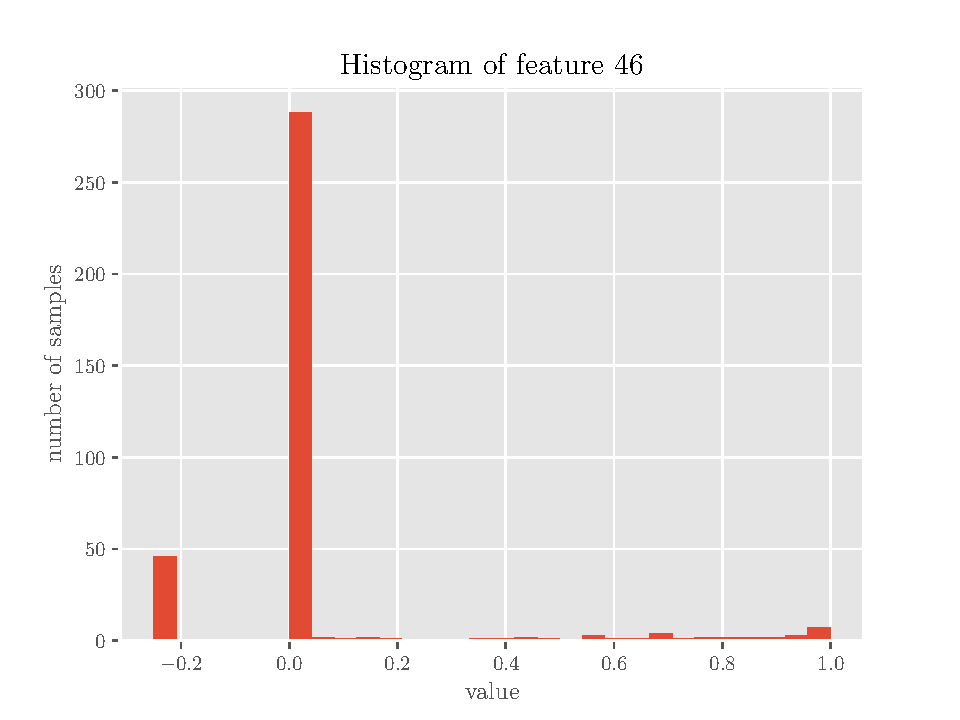
\includegraphics[scale=0.75]{fig_01.pdf}


We fit and retrain

\end{document}
